\documentclass{article}
\usepackage[utf8]{inputenc} % allow utf-8 input
\usepackage[T1]{fontenc}    % use 8-bit T1 fonts
\usepackage{hyperref}       % hyperlinks
\usepackage{url}            % simple URL typesetting
\usepackage{booktabs}       % professional-quality tables
\usepackage{amsfonts}       % blackboard math symbols
\usepackage{nicefrac}       % compact symbols for 1/2, etc.
\usepackage{microtype}      % microtypography
\usepackage{mathptmx}
\usepackage{xcolor}         % colors
\usepackage[left=1.5in, right=1.5in, top=1in]{geometry}
\usepackage{graphicx}
\usepackage{float}
\usepackage{placeins}
\usepackage{amsmath}
\usepackage{subcaption}
\usepackage[skip=0.5\baselineskip]{caption}

\author{
 \textbf{Guankai, Sang}\\
  Boston University
  \and
 \textbf{Yifan, Zhang}\\ 
 Boston University
}
\title{\rule{\textwidth}{4pt}\\\textbf{Sentiment Prediction through Deep Neural Network}\\\rule{\textwidth}{1pt}}
\begin{document}
\maketitle
\begin{abstract}
  Nowadays, people rarely have time to finish all movies, even the latest one, therefore movie reviews become a choosing standard. Having a high accuracy on sentiment prediction of movie reviews, people can save their time even more  by not reading each single review and still can know others' attitude on those movies. We trained a Multi-layer neural network with IMDB data imported from Keras. Even the dataset has been already processed, we still need to do word embedding and split validation dataset from training dataset. For increasing the accuracy of our model without overfitting, we changes parameters such as learning rate, epoch, and also adding more hidden layers with proper dropout rates between them. Finally, two-hidden-layer neural network with adjusted parameters not only gets a higher model accuracy around 95\% but also achieve a higher validation accuracy around 88\% before overfitting.
\end{abstract}
\section{Dataset Preparation}
\subsection{Review Length Limitation}	
To do a text classification, the first step of building a model is word embedding, which maps words in movie review to a high dimensional vector. Since all neural network requires to have input with same size, we need to truncate or pad the dataset before we do word embedding. 
\vspace{5.5pt}

\noindent Shown as Figure \ref{fig:length}, the mean of review length in IMDB dataset is 234.76 words and the standard deviation is 172.911. Also, we can see from the boxplot, that the maximum of the dataset is around 500. Therefore, even there are multiple outliers that have over 500 word length, we still can set the value of maxlen in pad\_sequences function as 500 to cover the most of dataset. Then, this function will take the original training and testing dataset and truncate reviews longer than 500 or pad reviews shorter than that with 0. 
\FloatBarrier
\begin{figure}[htb]
    \centering
    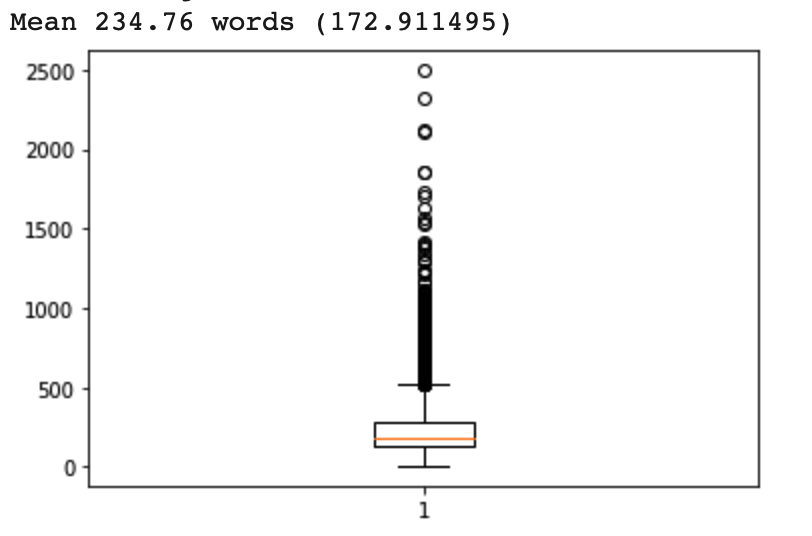
\includegraphics[width=5.5cm]{length}
    \caption{Distribution of review length in words}
    \label{fig:length}
\end{figure}
\FloatBarrier

\subsection{Validation Dataset}
A major challenge of training a neural network is overfitting, which means that a model acts so well on training dataset, but not on new coming dataset. One of way to solve it is through validation dataset in order to update parameters of model so that model will act well on general data. 
\FloatBarrier
\begin{figure}[htb]
\begin{subfigure}{.5\textwidth}
  \centering
  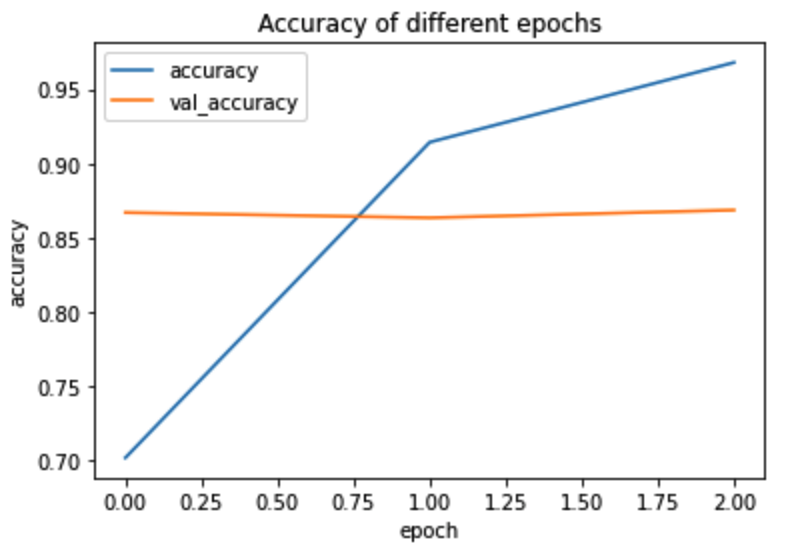
\includegraphics[width=6cm]{test as validation}
  \caption{Test dataset as validation}
  \label{fig: Test dataset as validation}
\end{subfigure}
\begin{subfigure}{.5\textwidth}
  \centering
  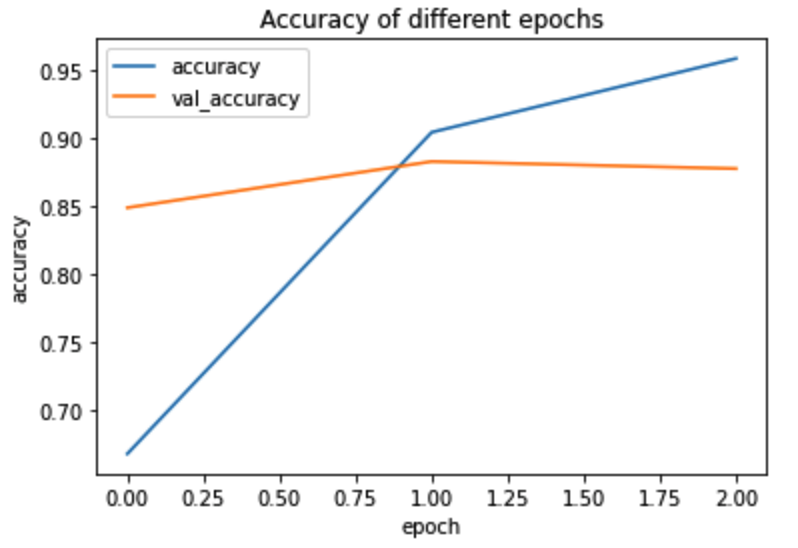
\includegraphics[width=6cm]{validation}
  \caption{With extra validation dataset}
  \label{fig:validation dataset}
\end{subfigure}
\caption{Accuracy of models with or without validation dataset}
\label{fig:Accuracy  val}
\end{figure}
\FloatBarrier
\noindent By training a multi-layer models with extra validation dataset or not, we can see the accuracy difference between them. Figure \ref{fig:Accuracy  val} shows that the validation accuracy of model with no extra validation decreases from the first epoch when the accuracy of the model continuously increases. However, the validation accuracy of model with extra validation dataset decreases after the first epoch. This means without extra validation dataset, model will become overfitting earlier. Also, shown as Table \ref{accuracy validation}, model with extra validation has the highest model accuracy. Therefore, in order to have enough training and validation dataset as the same time, we separate a half of training dataset as validation dataset after shuffling.
 \FloatBarrier
\begin{table}[htb]
\centering
\caption{Accuracy of models}
	\begin{tabular}{||c c c c ||} 
	 \hline
 	&No validation & Test dataset as validation& With extra validation \\ [0.5ex] 
 	\hline\hline
 	 Accuracy& 86.94 & 86.85 & 87.14 \\ 
 	\hline
	\end{tabular}
\label{accuracy validation}
\end{table}
\FloatBarrier

\section{Modeling and Optimization}
The starting model that we build has one word embedding layer, a flatten layer, and two dense layers. Output of embedding layer is 32×500, since we would like to have word vector in 32 dimensions and the input length at 500 as discussed previously. Activation for the hidden layer is Relu, and that for the output layer is Sigmoid in order to get results in percentage. Optimizer is Adam with learning rate 0.0005. Training this model in three epochs with extra validation dataset, we get model accuracy around 87\% and early overfitting. 
\subsection{Learning rate}
One of the way to avoid overfitting is picking a proper learning rate, which can help model get higher accuracy before overfitting appears. Shown as Figure \ref{fig:lr}, learning rate in 0.005, which is our starting learning rate, it has highest starting accuracy, and it can even reach closely to 1 at the end. However, from Table \ref{learning rate}, we can see that even model with learning rate 0.005 has highest model accuracy at the beginning, it gets overfitting earlies as well, and  when the accuracy at that time is just around 80\%. Among all the learning rate value, 0.0001 gives the best result. Its model accuracy  before overfitting is 94.42\%, which is the highest score than others. Therefore, we changes learning rate to 0.0001.

\FloatBarrier
\begin{figure}[htb]
    \centering
    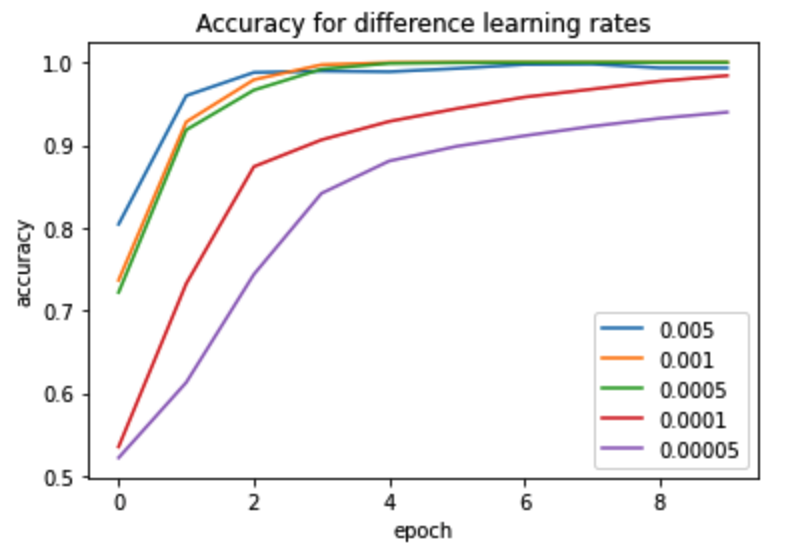
\includegraphics[width=6cm]{learningrate}
    \caption{Accuracy of different learning rate}
    \label{fig:lr}
\end{figure}
\FloatBarrier
\FloatBarrier
\begin{table}[htb]
\centering
\caption{Accuracy and validation accuracy of different learning rate}
	\begin{tabular}{||c c c ||} 
	 \hline
 	Learning rate&Overfitting appears at & Accuracy \\ [0.5ex] 
 	\hline\hline
 	0.005 & Epoch 2 & 0.8042\\
 	0.001 & Epoch 3 & 0.9281\\
 	0.0005 & Epoch 3 & 0.9184\\
 	0.0001 & Epoch 7 & 0.9442\\
 	0.00005 &  Epoch 10 &  0.9393\\               
 	\hline
	\end{tabular}
\label{learning rate}
\end{table}
\FloatBarrier

\subsection{Hidden layer}
Another way to increase the accuracy of the model is having deeper layer. However, having more layers also means more parameters and more complex model, which could cause overfitting. Therefore, choice on neuron number and balance between neuron and depth of the model becomes important.
\vspace{5.5pt}

\noindent By using EarlyStopping function with patience value 2, we will get the accuracy of the model before validation accuracy decreases too much, which caused by overfitting. The result is shown as Figure \ref{fig:Accuracy  hidden}. From part (a), we can clearly see that for the first layer, 10 neurons gives the highest accuracy before overfitting, and for the second layer, seeing from part (b), we get the highest accuracy with 12 neurons. In part (c), models with 14 neurons gives the best result. However, shown in Table \ref{acc_depth}, the validation accuracy of the model with either only one hidden layer or  three hidden layers is not as good as the model with two hidden layers. Therefore, we will only use two hidden layers, one with 10 neurons and the other with 12 neurons. 
\FloatBarrier
\begin{table}[htb]
\centering
\caption{Accuracy of different depth}
	\begin{tabular}{||c c c c||} 
	 \hline
 	layer number & neuron number& Model accuracy before overfitting & val\_accuracy\\ [0.5ex] 
 	\hline\hline
 	1 & 10 neuron & 0.9614 & 0.8695\\
 	2 & 12 neuron & 0.9526 & 0.8762\\
 	3 & 14 neuron & 0.9701 & 0.8618\\
 	\hline
	\end{tabular}
\label{acc_depth}
\end{table}
\FloatBarrier
\FloatBarrier
\begin{figure}[htb]
\begin{subfigure}{.5\textwidth}
  \centering
  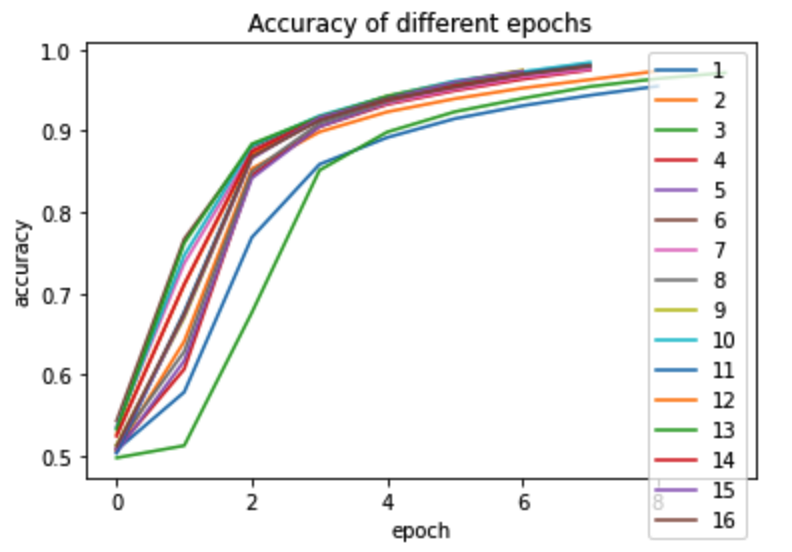
\includegraphics[width=5.5cm]{hidden1}
  \caption{Hidden layer 1}
  \label{fig: hidden1}
\end{subfigure}
\begin{subfigure}{.5\textwidth}
  \centering
  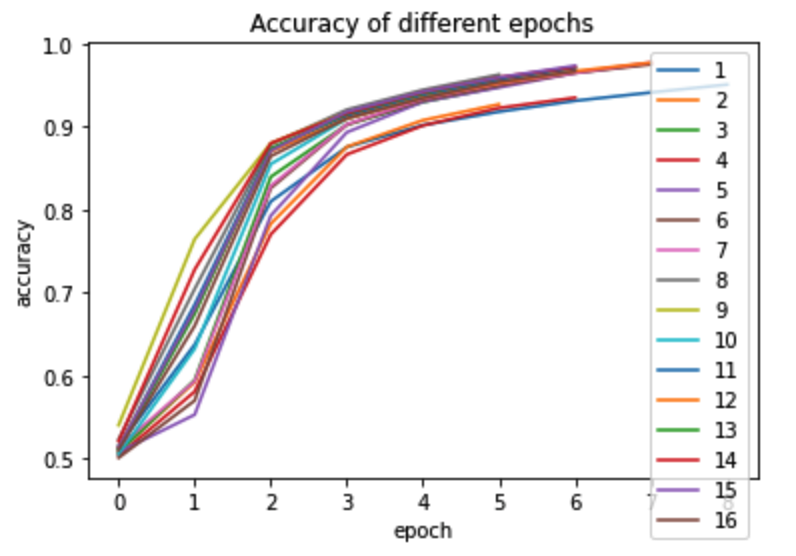
\includegraphics[width=5.5cm]{hidden2}
  \caption{Hidden layer 2}
  \label{fig:validation dataset}
\end{subfigure}
\begin{subfigure}{.5\textwidth}
  \centering
  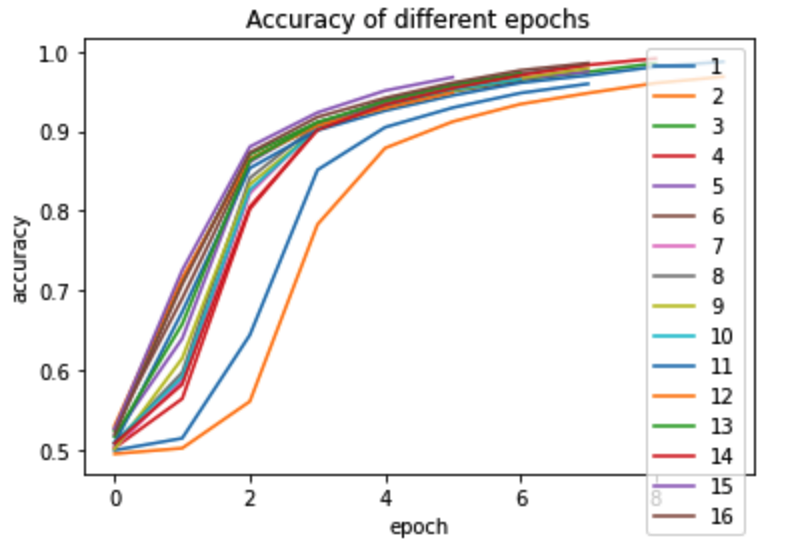
\includegraphics[width=5.5cm]{hidden3}
  \caption{Hidden layer 3}
  \label{fig: hidden3}
\end{subfigure}
\caption{Accuracy depended on neuron number in each layer}
\label{fig:Accuracy  hidden}
\end{figure}
\FloatBarrier
\subsection{Dropout}
Adding a dropout layer after dense layer helps prevent overfitting as well. Since it drops a percent of neurons due to the setting up dropout rate and then continue training the model, this add some randomness during the training process. Seeing from the Figure \ref{fig:dr}, we can see that our model achieve highest accuracy when dropout rate equals to 0.3, and the accuracy of the model is 0.9445 and validation rate is 0.8717. Since this does not give a higher model accuracy or validation accuracy, we will not use any dropout layer for our final model.
\FloatBarrier
\begin{figure}[htb]
    \centering
    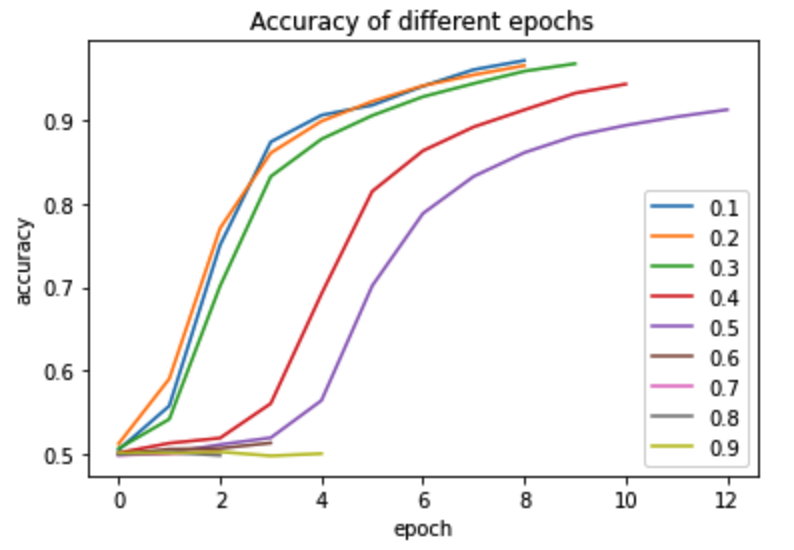
\includegraphics[width=6cm]{droprate}
    \caption{Accuracy with various dropout rate}
    \label{fig:dr}
\end{figure}
\FloatBarrier

\section{Conclusion}
The major challenge in our model is the decision on the proper review length as the input of word embedding layer and on the parameter in the deep neural network to avoid overfitting while increasing the model accuracy. Through the analysis of the distribution of general review length, we decide the input of word embedding layer as 500. Shown as Table \ref{final}, by manipulating learning rate, we increase the model accuracy significantly, and then by adding hidden layer, changing number of neurons and trying various dropout rate, we improve the validation accuracy while keeping the model accuracy around. Our final model has learning rate in 0.0001 with two hidden layer. The first hidden layer with 10 neurons and the second with 12 neurons. Even though we get high model accuracy as 0.9526 and validation model as 0.8741, it still can be further improved. In our model, we try to set each dropout layer with the same dropout rate, and it does not give us a better result, but for future improvement, we can make them different according to the specific output of the previous dense layer. We could also try to use 1D CNN based on our final model. 
\FloatBarrier
\begin{table}[htb]
\centering
\caption{The accuracy of all four methods}
	\begin{tabular}{||c c c||} 
	 \hline
 	Changes & Model accuracy & Validation accuracy\\ [0.5ex] 
 	\hline\hline
 	Basic Model & 0.7054 & 0.8709\\
 	learning rate & 0.9595 & 0.8741 \\ 
 	Depth of the model & 0.9526 & 0.8762\\
   	Dropout rate & 0.9445 & 0.8717\\
   	
 	\hline
	\end{tabular}
\label{final}
\end{table}
\FloatBarrier
\end{document}


